\documentclass[11pt]{article}
\usepackage[margin=1in]{geometry}
\usepackage{amsmath,amssymb,booktabs,graphicx,caption,subcaption,hyperref,xcolor,enumitem}
\usepackage{listings}
\hypersetup{colorlinks=true,linkcolor=black,urlcolor=blue!50!black}
\graphicspath{{../results/}{../results/dataset/}}
\setlist{nosep}
\lstset{basicstyle=\ttfamily\small,breaklines=true}
\newcommand{\pct}[1]{#1\,\%}

\title{Music Genre Classification from Spectrograms\\\large CNN trained on Deezer previews vs.\ CLAP embeddings}
\author{Karol D\k{a}browski \\ First-Year Seminar}
\date{28 October 2026}

\begin{document}
\maketitle

\begin{abstract}
A convolutional network classifies 30-second music clips into eight genres (classical, pop, jazz, hip-hop, rock, electronic, country, film score) from log-mel spectrograms. Data: 25\,943 previews scraped from the public Deezer API, labelled by album genre tag, split by artist. Best from-scratch CNN: \pct{77.4} test accuracy on unseen artists. A small classifier on frozen CLAP audio embeddings reaches \pct{79.4}; zero-shot CLAP \pct{69.4}. Chance is \pct{12.5}.
\end{abstract}

\section{Data}
\begin{itemize}
  \item Source: Deezer public API (no key). Spotify no longer serves audio previews.
  \item Per genre $g$ with Deezer genre id: seed artists from genre charts, editorial playlists and radios; breadth-first expansion over \texttt{/artist/\{id\}/related}.
  \item Keep artist $a$ iff $\;\frac{|\{\text{albums of } a \text{ with genre\_id}=g\}|}{|\text{albums of } a|}\ge 0.5$. Label of a track $=$ its album's genre id (must equal $g$).
  \item Caps: $\le 12$ tracks/artist, $\le 4$/album; artist in exactly one genre. Film score: genre ``Films/Games'' seeded from 65 film and game composers (genre charts skipped: pop songs from films).
  \item Split by artist, stratified per genre, 80/10/10. Second crawl (new artists only) doubled the training set; val/test clips unchanged.
  \item Fresh set: 504 clips, 258 artists absent from all splits, 63 per genre.
\end{itemize}
\begin{table}[h]\centering\small
\begin{tabular}{lrrrr}\toprule
 & clips & train & val & test \\\midrule
first crawl (cnn\_v3) & 12\,699 & 10\,214 & 1\,281 & 1\,204 \\
after extension (cnn\_v4) & 25\,943 & 23\,458 & 1\,281 & 1\,204 \\
fresh set & 504 & -- & -- & 504 \\\bottomrule
\end{tabular}
\caption{Dataset sizes. $\approx$1\,600 (later $\approx$3\,250) clips per genre.}
\end{table}
\begin{figure}[h]\centering
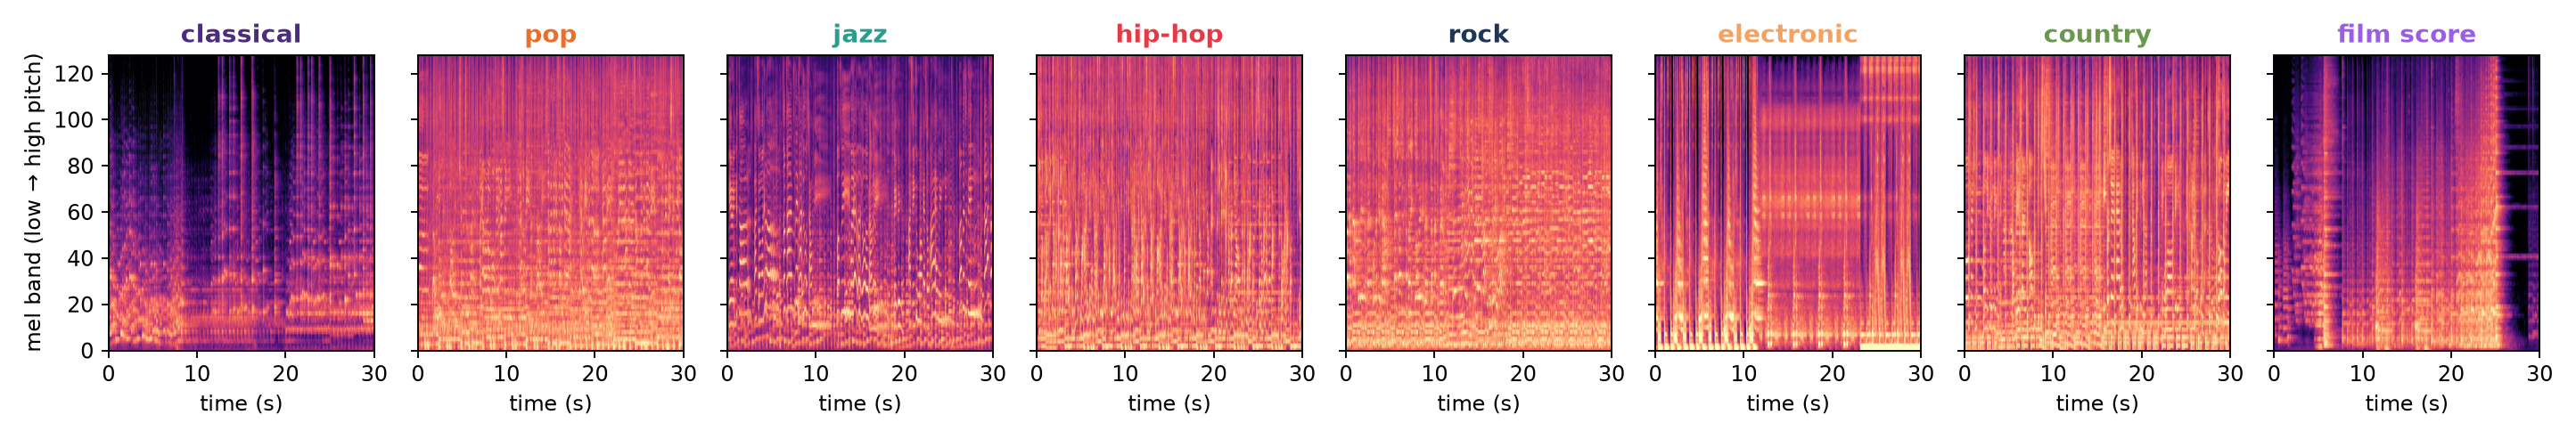
\includegraphics[width=\textwidth]{typical_spectrograms.png}
\caption{Most typical clip per genre (closest to the genre's mean spectrum), shared colour scale.}
\end{figure}

\section{Features}
Mono, resampled to $f_s=22\,050$\,Hz, 30\,s $\Rightarrow x\in\mathbb{R}^{661\,500}$.
\begin{align}
S[k,t] &= \Big|\sum_{n} x[n+tH]\,w[n]\,e^{-2\pi i kn/N}\Big|^2, \quad N=2048,\ H=1024 \\
M[m,t] &= \log\Big(\sum_k F_{m,k}\,S[k,t] + 10^{-6}\Big), \quad m=1,\dots,128,\ t=1,\dots,646
\end{align}
$F$: mel filterbank, 20\,Hz--11\,025\,Hz. Training input: random 10\,s crop (216 frames) $+$ SpecAugment (2 frequency masks $\le 16$ bins, 2 time masks $\le 10\%$) $+$ random gain. Evaluation: full 30\,s.
\begin{figure}[h]\centering
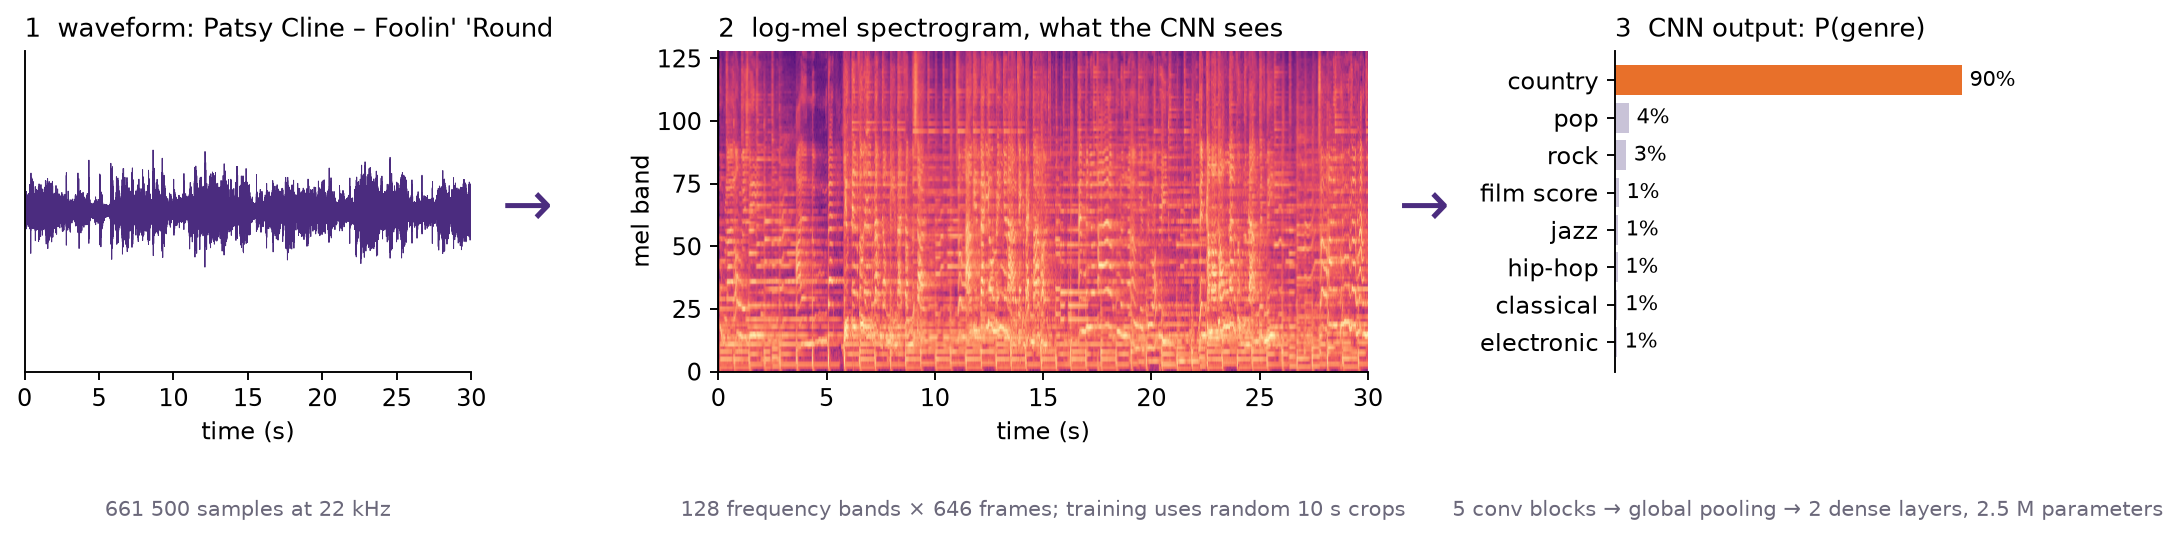
\includegraphics[width=\textwidth]{pipeline_example.png}
\caption{One test clip through the pipeline.}
\end{figure}

\section{Model}
\begin{table}[h]\centering\small
\begin{tabular}{llr}\toprule
layer & spec & output \\\midrule
input norm & BatchNorm(1) & $1\times128\times T$ \\
block $\times 5$ & $2\times[\text{conv }3{\times}3,\ \text{BN},\ \text{ReLU}]$, maxpool 2 & widths $w,2w,4w,8w,8w$ \\
pooling & concat(global avg, global max) & $16w$ \\
head & dropout 0.3, FC 256, ReLU, dropout 0.3, FC 8 & 8 \\\bottomrule
\end{tabular}
\caption{VGG-style CNN. $w=32$: 2.49\,M parameters (cnn\_v3); $w=48$: 5.49\,M (cnn\_v4).}
\end{table}
\begin{align}
\mathcal{L} &= -\sum_{c} \tilde y_c \log p_c, \qquad \tilde y_c = (1-\epsilon)\,\mathbb{1}[c=y] + \epsilon/8,\quad \epsilon=0.1 \\
\text{class weight}_c &\propto (N/n_c)^{1/2}
\end{align}
AdamW, lr $10^{-3}$, weight decay $10^{-2}$, one-cycle schedule, batch 64. cnn\_v3: $w=32$, 40 epochs on 7 genres then 9 epochs fine-tuned with a new 8-way head. cnn\_v4: $w=48$, 11 epochs from scratch on the extended data.

\section{CLAP baselines}
CLAP (LAION, \texttt{laion/larger\_clap\_general}): audio encoder $f_a$ and text encoder $f_t$ into $\mathbb{R}^{512}$, trained contrastively on audio--caption pairs.
\begin{align}
\mathbf{a} &= \frac{1}{3}\sum_{j=1}^{3} f_a(x_j),\quad x_j = \text{10\,s chunk } j\ \text{(48\,kHz)} \\
\mathbf{t}_c &= \operatorname{mean}_{s\in\mathcal{S}_c} f_t(s),\qquad \mathcal{S}_c = \{\text{2 descriptions} \times \text{3 templates}\} \\
p_c &= \operatorname{softmax}_c\!\Big(\tau \,\frac{\mathbf{a}\cdot\mathbf{t}_c}{\|\mathbf{a}\|\,\|\mathbf{t}_c\|}\Big),\qquad \tau = e^{\text{logit\_scale}_a}\approx 39 \quad\text{(zero-shot)} \\
\hat p &= \operatorname{softmax}\big(W_2\,\mathrm{GELU}(W_1\,\hat{\mathbf{a}})\big),\quad \hat{\mathbf{a}}=(\mathbf{a}-\mu)/\sigma,\ W_1\in\mathbb{R}^{256\times512},\ W_2\in\mathbb{R}^{8\times256} \quad\text{(head)}
\end{align}
Head: CLAP frozen; dropout 0.5, AdamW wd 0.1, 300 epochs, cosine lr; hidden size and regularisation chosen on val. Trained on the 10\,214 first-crawl clips. Ensemble $=$ mean of cnn\_v4 and head probabilities.

\section{Results}
\begin{table}[h]\centering\small
\begin{tabular}{lrrrrr}\toprule
 & params trained & test acc & test F1 & fresh acc & fresh F1 \\\midrule
cnn\_v3 ($w=32$, 10k train clips) & 2.5\,M & 0.754 & 0.754 & 0.778 & 0.778 \\
cnn\_v4 ($w=48$, 23k train clips) & 5.5\,M & 0.774 & 0.773 & 0.794 & 0.794 \\
CLAP zero-shot & 0 & 0.694 & 0.696 & 0.728 & 0.728 \\
CLAP embeddings $+$ classifier & 0.13\,M & 0.794 & 0.791 & 0.813 & 0.814 \\
ensemble cnn\_v4 $+$ head & -- & \textbf{0.797} & \textbf{0.795} & \textbf{0.815} & \textbf{0.814} \\\bottomrule
\end{tabular}
\caption{Accuracy and macro-F1, 8 classes. Test: 1\,204 clips, artists unseen in training. Fresh: 504 clips, 258 new artists. Chance $=0.125$.}
\end{table}
\begin{table}[h]\centering\small
\begin{tabular}{lrrr|rrr}\toprule
 & \multicolumn{3}{c|}{test F1} & \multicolumn{3}{c}{fresh F1} \\
genre & cnn\_v4 & head & ens. & cnn\_v4 & head & ens. \\\midrule
classical & 0.81 & 0.82 & 0.82 & 0.86 & 0.82 & 0.87 \\
pop & 0.62 & 0.65 & 0.67 & 0.59 & 0.69 & 0.62 \\
jazz & 0.80 & 0.81 & 0.82 & 0.84 & 0.83 & 0.85 \\
hip-hop & 0.85 & 0.91 & 0.90 & 0.93 & 0.95 & 0.95 \\
rock & 0.76 & 0.77 & 0.76 & 0.81 & 0.78 & 0.83 \\
electronic & 0.75 & 0.80 & 0.78 & 0.70 & 0.84 & 0.73 \\
country & 0.88 & 0.88 & 0.90 & 0.87 & 0.81 & 0.87 \\
film score & 0.71 & 0.70 & 0.72 & 0.75 & 0.79 & 0.79 \\\bottomrule
\end{tabular}
\caption{Per-genre F1.}
\end{table}
\begin{figure}[h]\centering
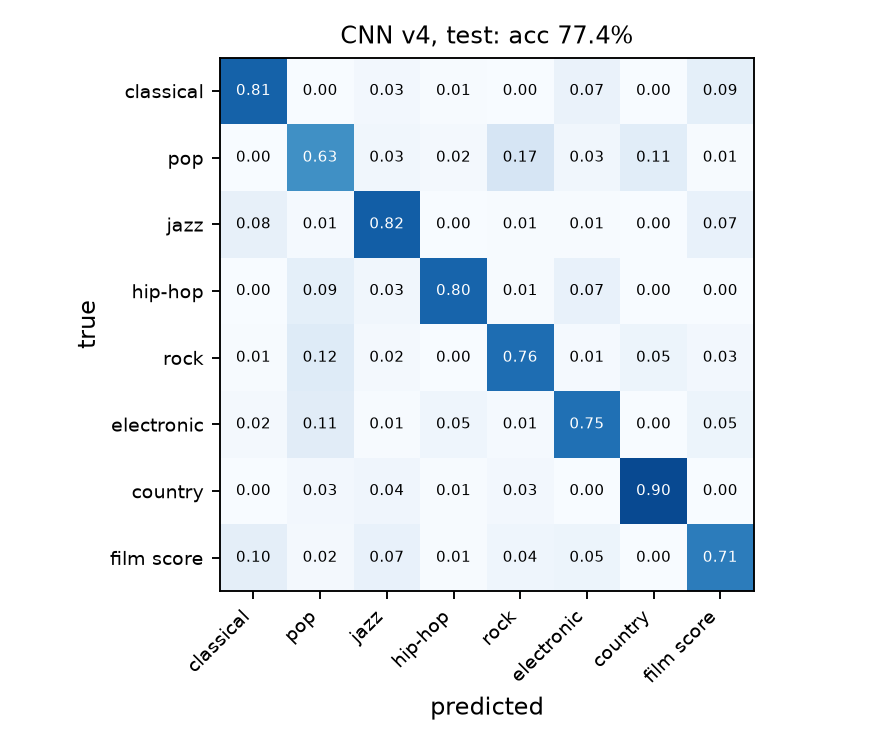
\includegraphics[width=.49\textwidth]{confusion_cnn_v4_w48_test.png}\hfill
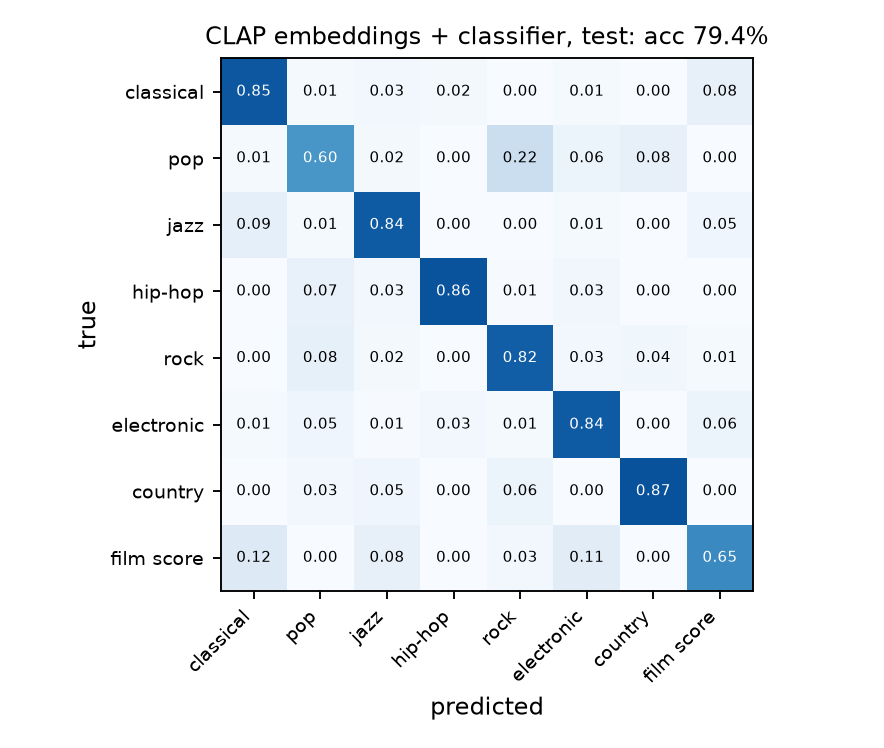
\includegraphics[width=.49\textwidth]{confusion_clap_head_test.png}
\caption{Row-normalised confusion matrices on the test split.}
\end{figure}
\begin{table}[h]\centering\small
\begin{tabular}{lrrrrrr}\toprule
clip length & 2\,s & 3\,s & 5\,s & 10\,s & 15\,s & 30\,s \\\midrule
cnn\_v3 test acc & 0.520 & 0.622 & 0.674 & 0.750 & 0.735 & 0.756 \\\bottomrule
\end{tabular}
\caption{Accuracy vs.\ centre-cropped test clip length.}
\end{table}
\begin{figure}[h]\centering
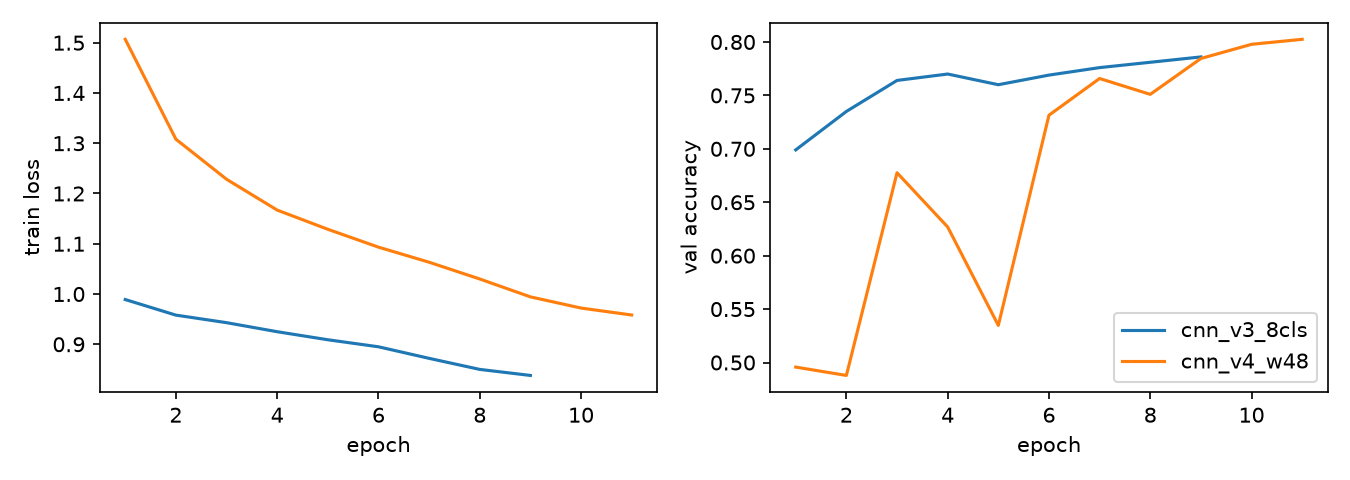
\includegraphics[width=.62\textwidth]{curves_cnn_v3_8cls_cnn_v4_w48.png}
\caption{Training curves. cnn\_v3 shown for its 9 fine-tuning epochs.}
\end{figure}

\section{Observations}
\begin{itemize}
  \item Pop is the catch-all: cnn\_v4 sends \pct{11} of pop to rock and \pct{13} to country; rock, hip-hop, electronic each leak \pct{10}--\pct{14} into pop. Label-level ambiguity, not fixable by data.
  \item Classical $\leftrightarrow$ film score: \pct{20} of classical predicted as score. Adding the 8th class cost classical recall $0.90\to0.67$ (cnn\_v2 $\to$ cnn\_v3).
  \item Doubling data $+$ 2.2$\times$ parameters: $+2.0$ pts test, $+1.6$ pts fresh. Val still rising at the last epoch.
  \item Transfer beats scratch: 0.13\,M trained parameters on frozen CLAP embeddings $>$ 5.5\,M-parameter CNN on 2$\times$ data. Ensemble adds $+0.3$ pts: both models fail on the same clips.
  \item Zero-shot CLAP calls 40/63 fresh electronic clips pop; depends on prompt wording (untuned).
  \item Published human agreement on broad genre labels $\approx$ 0.75--0.85: the models are near the label-noise ceiling.
\end{itemize}

\section{Limitations and next steps}
\begin{itemize}
  \item Labels are album-level Deezer tags; 30\,s previews, not full songs.
  \item \texttt{laion/larger\_clap\_music} loads with a degenerate logit scale under transformers 5; not evaluated.
  \item Next: tune CLAP prompts on val; longer schedule for cnn\_v4; fine-tune the CLAP audio encoder end-to-end; 100k clips ($\approx$ 1 day: 48\,GB, streaming loader, $w=64$).
\end{itemize}

\section*{Code}
\texttt{\textasciitilde/Desktop/College/FYS/genre/src}: \texttt{scrape\_deezer.py}, \texttt{extend\_data.py}, \texttt{crawl\_score.py}, \texttt{preprocess.py}, \texttt{train.py}, \texttt{evaluate.py}, \texttt{clap\_zero.py}, \texttt{clap\_embed.py}, \texttt{clap\_head.py}, \texttt{eval\_all.py}, \texttt{fresh\_test.py}, \texttt{app.py} (demo UI).
\begin{lstlisting}
python src/scrape_deezer.py && python src/preprocess.py
python src/train.py --name cnn_v4_w48 --width 48 --epochs 11
python src/clap_embed.py && python src/clap_head.py
python src/eval_all.py cnn_v4_w48 clap_head "ensemble:cnn_v4_w48+clap_head"
\end{lstlisting}
\end{document}
